\documentclass[10pt]{article}
\usepackage[utf8]{inputenc}
\usepackage[T1]{fontenc}
\usepackage{graphicx}
\usepackage[export]{adjustbox}
\graphicspath{ {./images/} }
\usepackage{amsmath}
\usepackage{amsfonts}
\usepackage{amssymb}
\usepackage[version=4]{mhchem}
\usepackage{stmaryrd}
\usepackage{caption}

\begin{document}

\section*{1 Gravitational wave astronomy (45 points)}
In this problem, we will analyze frequency vs time representations of data containing the gravitational wave event GW170817, which was the first observation by LIGO of a merger of a binary neutron star system.\\
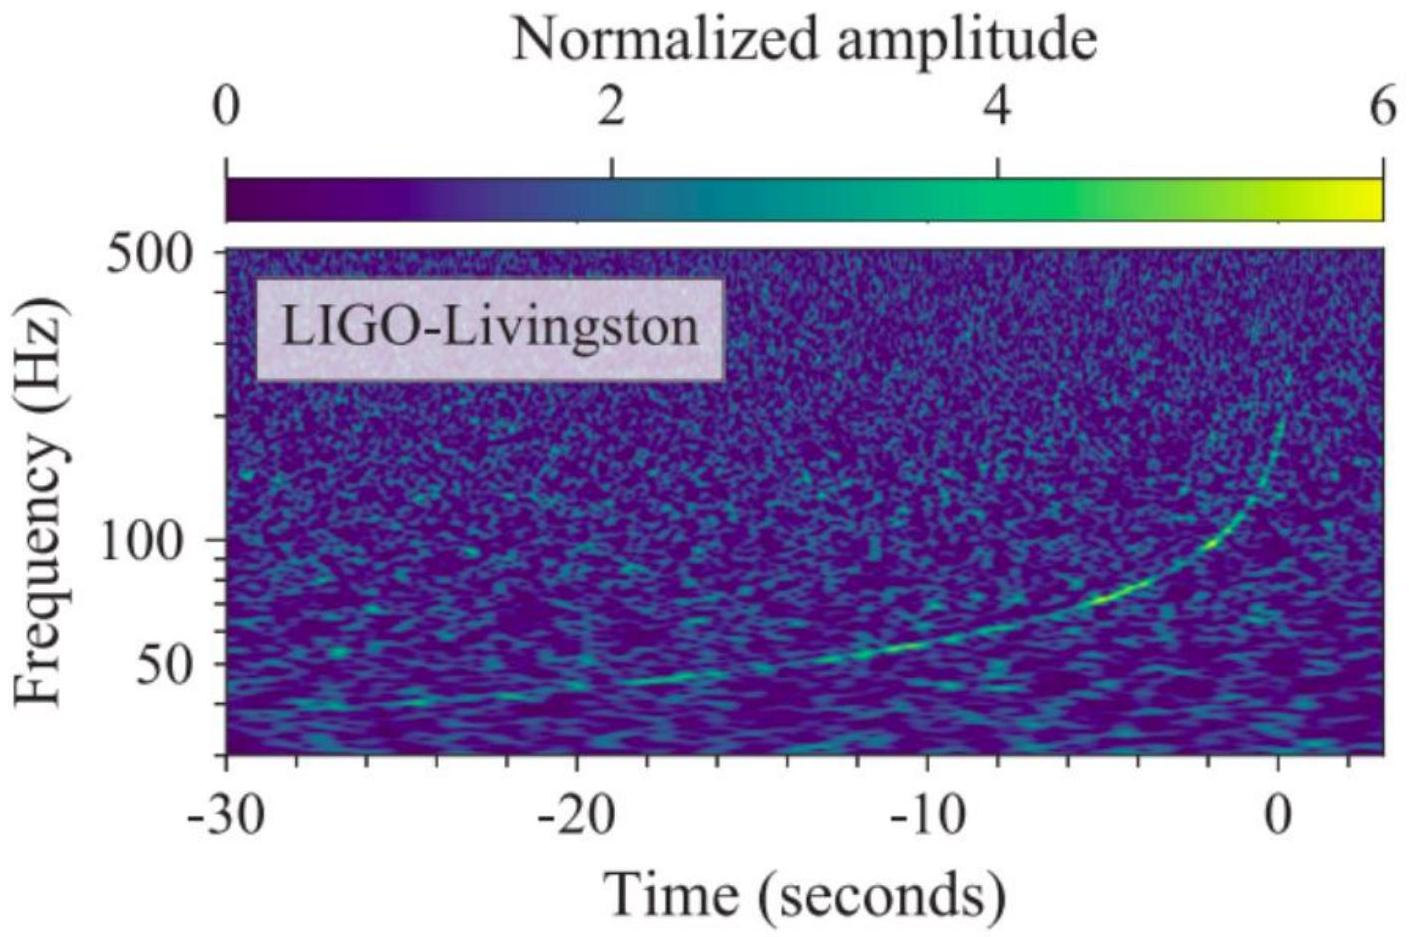
\includegraphics[max width=\textwidth, center]{2025_09_11_3681df2e94a9f94ef296g-2}

\subsection*{1.1 Data from the graph}
1.1.1 You are given a semi-logarithmic graph, from which you need to extract values of frequency and time. Let bottom left corner be origin ( 0,0 ), horizontal coordinate $x$ is measured in centimeters. Find a linear expression to obtain actual time $t$ from $x$.\\
1.1.2 Similarly, find an expression for the frequency $f$ as a function of the vertical coordinate $y$ measured in centimeters.\\
(3pt)\\
1.1.3 Extract 14 values of time and corresponding frequency from the given graph into a table. At least one of the values should correspond to a frequency more than 100 Hz . (7pt)

\subsection*{1.2 Calculate system parameters}
The most plausible explanation for this evolution of frequency is the in-spiraling of two orbiting masses, $m_{1}$ and $m_{2}$, due to gravitational-wave emission. At the lower frequencies, such evolution is characterized by the "chirp mass"

$$
M_{\text {chirp }}=\frac{\left(m_{1} m_{2}\right)^{3 / 5}}{\left(m_{1}+m_{2}\right)^{1 / 5}}=\frac{c^{3}}{G}\left[\frac{5}{96} \pi^{-\frac{8}{3}} f^{-\frac{11}{3}} \dot{f}\right]^{\frac{3}{5}}
$$

where $f$ and $\dot{f}$ are the observed frequency and its rate of change with respect to time, and $G$ and $c$ are the gravitational constant and speed of light.\\
1.2.1 From the equation above, derive an expression for the frequency dependence on time.\\
(3pt)\\
Note: if $x^{n} \dot{x}=k$, then $\frac{x^{n+1}}{n+1}=k t+C$, where $k, n$ and $C$ are constants.\\
1.2.2 By plotting the appropriate graph, find the chirp mass and estimate its error caused by uncertainty in slope calcilation.\\
(22pt)

We realize that what is measured by the ground-based GW detectors are actually the detector-frame masses, which are related to the source frame masses by

$$
m_{\text {detector }}=(1+z) m
$$

where $z$ is the redshift of the binary.\\
1.2.3 If the host galaxy NGC 4993 has a redshift $\mathrm{z}=0.009783$, find the source frame chirp mass.\\
(2pt)\\
1.2.4 The mass ratio $q=\frac{m_{1}}{m_{2}}$, is much harder to measure. Advanced waveform analysis shows that $q$ for this system was in the range of 0.73 to 1.0 . Calculate range of values for the masses $m_{1}$ (primary) and $m_{2}$ (secondary).\\
(6pt)

\end{document}